\documentclass{article}
\usepackage{tikz}

\begin{document}

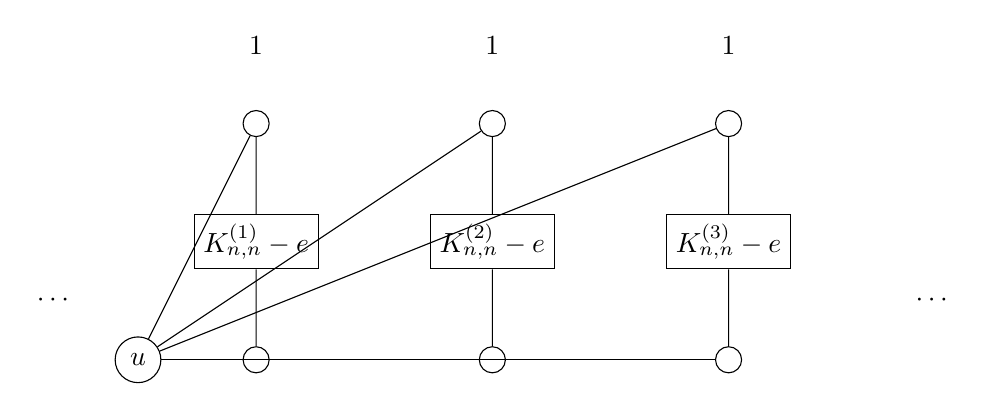
\begin{tikzpicture}[scale=1.5]
    % Define the nodes
    \node (u) at (0, 0) [circle, draw] {$u$};
    
    % Define the subgraphs
    \foreach \i in {1,...,3} {
        \node (K_{n,n}^{(\i)}) at (\i * 2 - 1, 1) [rectangle, draw] {$K_{n,n}^{(\i)} - e$};
        \node (K_{n,n}^{(\i)}_1) at (\i * 2 - 1, 2) [circle, draw] {};
        \node (K_{n,n}^{(\i)}_2) at (\i * 2 - 1, 0) [circle, draw] {};
        
        \draw (K_{n,n}^{(\i)}_1) -- (K_{n,n}^{(\i)});
        \draw (K_{n,n}^{(\i)}_2) -- (K_{n,n}^{(\i)});
    }
    
    % Draw the edges connecting the subgraphs to u
    \foreach \i in {1,...,3} {
        \draw (K_{n,n}^{(\i)}_1) -- (u);
        \draw (K_{n,n}^{(\i)}_2) -- (u);
    }
    
    % Label the vertices
    \foreach \i in {1,...,3} {
        \node at (\i * 2 - 1, 2.5) [above] {$1$};
    }
    
    \node at (-0.5, 0.5) [left] {$\cdots$};
    \node at (6.5, 0.5) [right] {$\cdots$};
\end{tikzpicture}

\end{document}